\chapter[The Guilded Orrery]{Cosmology}
\label{cosmology}

\section{The Unstoppable Stars}

\label{astronomy}
\label{seasons}
\index{Seasons}
\index{Cycles}
\index{Astronomy}
\index{Time Parallel}

\boxPair{
  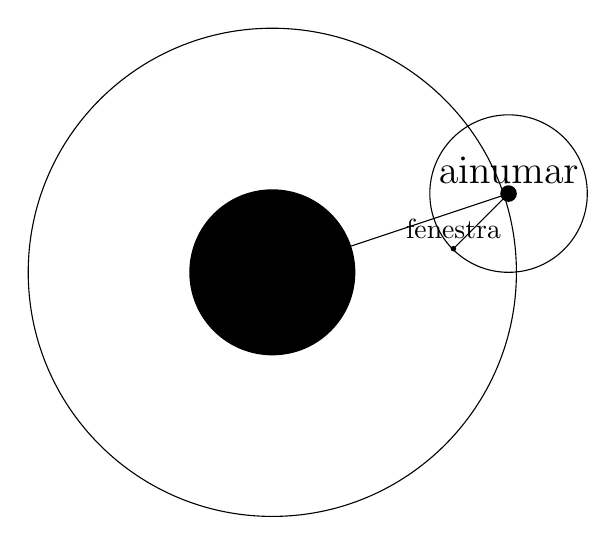
\begin{tikzpicture}
    \coordinate (S) at (0,0);
    \coordinate (A) at (3,1);
    \coordinate (F) at (2.3,0.3);
    \draw[\pageSideColor] (S) -- (A) -- (F);
    \draw[\pageSideColor] (S) circle (3.1);% Orbit
    \draw[\pageSideColor] (A) circle (1);% Suborbit
    \fill[\pageSideColor] (S)  circle (30pt);
    \fill[\pageOppositeColor] (A.south)  circle (3pt);
    \fill[\pageOppositeColor] (F.east) circle (1pt);
    \coordinate [label={\scshape\huge \outline{Sun}}] (S.south) at (0,0);
    \coordinate [label=\outline{\Large \glsentrytext{ainumar}}] (A) at (3,1);
    \coordinate [label=\outline{\glsentrytext{fenestra}}] (F) at ++(2.3,0.3);
  \end{tikzpicture}

}{
  \index{Qualmea}
  \index{Atya}
  \index{Alassea}
  \index{Cantea}
  \index{Calea}
  \index{Verea}
  \index{Otsea}
  \index{Toldea}
  \index{Laiquea}
  \index{Quainea}
  \index{Minquesta}
  \index{Ohta}
  \begin{nametable}[l|Y|c|Y]{Seasons}

    \textbf{Real Month} & \textbf{Far Season} & \textbf{Climate} & \textbf{Event} \\
    \hline
    \hline
    \showSeasonLine{1}
    \showSeasonLine{2}
    \showSeasonLine{3}
    \showSeasonLine{4}
    \hline
    \showSeasonLine{5}
    \showSeasonLine{6}
    \showSeasonLine{7}
    \showSeasonLine{8}
    \hline
    \showSeasonLine{9}
    \showSeasonLine{10}
    \showSeasonLine{11}
    \showSeasonLine{12}

  \end{nametable}
}

\setcounter{season}{\month}

\begin{multicols}{2}


\subsection{Parallel Time}
\index{Parallel Time}
\index{Seasons}

\Gls{fenestra}'s time keeps moving, just as ours does, but slightly faster.
For every week which passes in our world, three weeks pass over there, so after a single month here, \gls{fenestra} experiences a full season.

While we have \trackMonth, \gls{fenestra} has `\showSeason' -- a \showTemperature\ season.
Just as we have twelve months, \emph{they} have twelve seasons.

After three years, all twelve seasons have passed and a new cycle begins.
\Gls{fenestra}'s inhabitants track `cycles' more often than years, unsurprisingly.

\subsection{Astronomy}

The planet \gls{ainumar} shines bright in the night sky, and appears a little larger than our moon does to us.
A raging storm moves across its face, which can be seen about half of the cycle.
Many people believe that the gods live there, inside the moving eye of the storm.

Three moons circle the planet.
One shines yellow, another grey, and the third is our \gls{fenestra}.

Our worldmoon swings wildly around \gls{ainumar}, coming so close in that it could almost kiss the gods, and then hurtles back to sit in empty space, far away from the Sun.
Every trip around \gls{ainumar} lasts around a year.
After three years, \gls{ainumar} completes a `cycle', and the twelve seasons begin again.

The first season is called `Qualmea'.
It is full of brutal storms and earthquakes, active volcanoes explode, trees and buildings topple, then at its height, a planetary eclipse emerges, called `the shadow of the gods', and the world goes black in the middle of the day.

After this comes `Atya' -- a milder season -- then a deep cold season known as `Alassea', when people cheer themselves up by playing pranks, telling jokes and drinking or smoking to excess; at night, both \gls{ainumar} and the Sun become a little smaller.
Things settle down again for Cantea, the fourth season, though \gls{ainumar} remains distant as the first cycle ends.

The second cycle begins with a warm, Summery season called C\'{a}lea; during the night Fenestra, spins round to view a dazzling \gls{ainumar}.
The world's shadow races across the face of the home of the gods, creating a `dark eye'.
All the ice in the planet recedes to nothing, and soon it becomes so warm that people hide under the shade.
Nobody travels with armour during this time -- full body-coverings in the scorching heat would mean death by heatstroke.

On and on it spins, and only the creatures underground live with any kind of consistency.

\subsection{Events}
\index{Astrology}
Various cosmological and meteorological events boost people's abilities to cast spells -- even those who had none before.
These bonuses stack with \glspl{ingredient}, so someone with the right know-how can (and do) stand under the unnatural darkness of an eclipse, holding the ground-up remains of a stirge queen, with auroch hooves boiled to melting point, at the top of a mountain, screeching about opening a portal from a distant \gls{village} to an underground realm.%
\footnote{High level spells sometimes need to target something beyond the horizon.
As a result, spellcasters often have to traipse up mountains in order to cast their biggest spells.}

\subsubsection{Cold Snap}
\index{Cold Snap}
\index[mana]{Fate!Cold Snaps}

Cold snaps drain the life from characters and wildlife in a blink.
Until the weather warms up again, all actions outdoors inflict an additional \gls{fatigue} or more, depending on clothing.
Someone journeying outdoors effectively naked will receive 4 \glspl{fatigue}, per \gls{interval}.

The mass disturbances in the air, mixed with the darkness, creates a kind of magic in the air, which grants +1 to everyone's Fate Sphere, including those who cannot normally cast spells.

\subsubsection{Earthquakes}
\index{Earthquakes}
\index{Quakes}
\index[mana]{Earth!Quakes}

When the ground shakes, \gls{village} walls often fall, houses can topple inward, and gnomish warrens have their planning tested from the foundations to the rooves.
Despite the shaking, most structures remain standing.
Architects in \gls{fenestra} design castles to remain standing, despite the quakes, and dwarvish settlements at the edge of the \gls{deep} often feel nothing, as underground caverns don't shake during quakes as badly as the surface does.

When quakes alter rock, everyone with the tiniest understanding of magic finds themselves able to speak to stone, at least a little, as rocks and ice start to wake up.
This time grants a +1 bonus to everyone's Earth Skill, for the short duration of the quake.

The average person makes little use of this time -- they have more pressing concerns given the sudden lack of Sunlight.
But casters often plan grand rituals to coincide with an eclipse, as the extra powers allow them to perform wide-ranging, potent spells.

\subsubsection{Eclipses}
\index{Eclipses}
\index[mana]{Air!Eclipses}

When \gls{fenestra} passes behind the \gls{ainumar}, the Sun remains covered for hours.
For this entire \gls{interval}, the winds becomes more pliable, and anyone with a voice to speak gains +1 to their Air Skill.

\subsubsection{Floods}
\index{Floods}
\index[mana]{Water!Floods}

Floods can often damage infrastructure worse than earthquakes.
They rot food, and degrade the foundations of houses in subtle ways, which only become apparent years later.
While high fortifications can remain untouched, and underground dwelling runs the risk of water pouring in from above, driving everything inside up into the Sunlight.

The various predators of \gls{fenestra} seem to have an instinct for floods, and will camp outside any homely holes in their territories.

Travel during a flood poses serious problems -- any affected area will half the travellers' rate of movement.

While floods occur, everyone gains a +1 Bonus to their Water Skill, including those who began with 0.

\subsubsection{Heatwaves}
\index{Heatwaves}
\index[mana]{Fire!Heatwaves}

At the height of the warm seasons, heatwaves arrive and make \gls{fenestra} deadly, especially for the \gls{guard}.
All travel in direct Sunlight will have the travellers endure an additional +2 \glspl{fatigue} when wearing loose-fitting clothing, or +4 when wearing inappropriate clothes.
Armour of any kind does not count as `appropriate', so a heatwave can force any warrior to remove their armour.

During a heatwave, everyone gains a +1 bonus to their Fire Skill.

\subsubsection{Snow}
\index{Snow}

Snow halts travel.
Travelling over snow-covered lands reduces the standard travel by a third, then a half if snow falls again.
So when the troupe wants to travel 8 miles over road, they take the usual 4 \glspl{fatigue}, but only cover 6 miles after the snow falls.
Once more falls, they would only cover 4 miles.

\end{multicols}

\section{Guilded Temples}

\newcommand\guildRank[1]{\item[#1]\index{#1 (Rank)}}

\begin{multicols}{2}

\label{godsOfDeath}

\noindent
As any idiot can plainly see, the gods do not love humanity.
They treat people like children playing with insects.
And when a god finally kills someone, they claim that human soul for their realm.
Death by cold means joining \gls{sable}'s frozen realm, and death by violence allows \gls{wrecan} to pull the soul into her realm of eternal violence.

So when humanity looks to the divine, they do not look for salvation, but for danger.
Temples exists to protect civilization from the wrath of their god.

The temples are guilds with a divinely mandated monopoly, and each guild hall also serves as a temple.
Even a `guild hall' which is nothing more than an old lady's house still offers divine guidance.
The Temple of Hate encourages reconciliations, the Temple of Frost offers warmth, and the \gls{guard} work for the Temple of Beasts, where they kill the \gls{sylf}'s children.

\newcommand\guild[8]{
  \renewcommand\npcsymbol{#2}
  \vspace{2em}
  \noindent
  \begin{minipage}{\linewidth}
  \subsection[The Temple of #3]{#2~#1~#2 \\ \& \\ The Temple of #3}
  \ifdefmacro{#1}{}{\index{#1}\label{god:#1}}
  \index{#3 (God)}\label{god:#3}
  \ifdefmacro{#7}{}{\index{#7}\label{guild:#7}}
  \index{Gods}

  \begin{exampletext}
  \noindent
  #4
  \end{exampletext}
  \end{minipage}

  \noindent
  \begin{minipage}{\linewidth}
  \begin{description}
  \item[Domain:] #5

  \item[Defence:] #6

  \item[Watchers:] #7

  \item[Activities:] #8

  \end{description}
  \end{minipage}

  \subsubsection{#7}
}

\guild{\Glsfmttext{abderian}}% Name
  {\gls{poison}}% Symbol
  {Poison}% Death
  {
    Led doors, covered in ivy, open to usher in a city \gls{warden}, still dressed in the finery he wore for feasts in life.

    ``I told my daughter to bury me in my dinner jacket.
    I always knew she was the good sort'', he smiled.

    A tall and impossibly thin woman balances a wine class between two fingers and hands it to him.

    ``So what's for dinner in this noble realm?'', but the smile turns to a stare half way through a swig of wine, as he scans the room, and notes all the filthy beggars staring at their wine, without drinking it.

    {\sffamily ``We have some nobility''}, she says thoughtfully.
    {\sffamily ``We even have kings, from the olden days''}, pointing to a skin-clad skeleton, trying to lift a crown from the floor.

    The \gls{warden} chokes and coughs, and notes the specks of blood on his dinner jacket.

    ``Is this wine poisoned?!''

    {\sffamily ``All wine is poison.
    We just drink it stronger here.''}
  }% God
  {poisons, rot, mould, fungus, ale, feasts}% Domain
  {salt, distillation, rendering, vinegar, and wine}% Defence
  {\Glspl{server}}% Watchers
  {
    Brewing, and baking.
  }% Guild activities

Every \gls{warden} has one in their kitchen, and every town has a bakery near their slums.
They provide bread for the hungry, and beer for the sober.
Despite this, very few appreciate the guild.

The \glspl{warden} complain that they insist on a monopoly on cooking \emph{in every \gls{warden}'s home}, and \glspl{warden} who refuse end up poisoned sooner rather than later.
But the \gls{wheatGuild}%
\footnote{`The Temple of Poison', hardly makes for good advertising. The Guild still fiercely maintain their divine battle to ensure food safety, but they always identify as a `temple of wine', or 'brotherhood of beer', or similar.}
are quick to note that nobody with an official \gls{wheatGuild} cook has ever succumbed to poison, so this only shows that everyone should employ one.

\subsubsection{Structure}

\begin{description}
  \guildRank{Bakers}
  come from the streets, and generally return after a few months.
  The working hours and heat in the kitchens tire even the fittest of humans.
  \guildRank{Tenders}
  tend the bars, if they can curry enough favour to move away from baking.
  \guildRank{Cooks}
  require a good nose, fast hands, and enough savings to bribe their way into the position.
  \guildRank{Keepers}
  need fast eyes to read and tabulate books.
  They test every bottle, and remember the daily-changing price of every drink.
  They also test or switch their bottles to make sure they don't leave any shoes for someone else to step into, as nobody from the streets can imagine a better position than being a keeper.
  \guildRank{Landlords}
  renounce any official status as \glspl{warden}, buy a property, and join the guild near its top rank.
  They purchase supplies, barter with traders for wholesale prices, and keep in contact with the cooks who work with \gls{warden}.
  \guildRank{Cooks}
  know all the guild's best recipes, both for food and poison.
  Besides their special recipes, they do not in fact cook very much, as they too come from \gls{warden} families, and have better things to do.
\end{description}

\subsubsection{Temple Taverns}

Not every tavern is a temple, but the bigger the town, the more keen the \gls{wheatGuild} will feel on establishing themselves in the area.

\guild{Eldren}% Name
  {\gls{sickness}}% Symbol
  {Sickness}% Death
  {
    Approaching the doors, the sick may find a woman with her left arm and leg missing, and an older man with downs syndrome, ushering them into large, open halls, full of beds where people chat.

    Moving inside, a long hallways presents doors, where less comfortable residents try to die peacefully.
    Unfortunately the temple forbids alcohol, as they do not want to risk a single soul to death by poison.
    The gods have their own laws and technicalities.

    Those who reach the end unharmed can let their soul fall out peacefully.
    Death by old age guarantees a place with the peaceful dead, in \gls{eldren}'s realm.
  }% God
  {pensions, disability, family, and ancestry}% Domain
  {none}% Defence
  {\Glspl{helper}}% Watchers
  {
    Caring for the old, sick and infirm.
  }% Guild activities

Parents with disables children try to have their children work as a helper, rather than joining the \gls{guard}.

Most live their lives inside a city, not far from their temple.
A rare few travel around neighbouring \glspl{village}, checking for anyone who cannot handle the hard physical labour in the outer \glspl{village}.

Where other temples focus on finances, followers of \gls{eldren} serve their communities well, and always receive respect from people.
They say that killing a member of the Temple of Sickness brings a curse which lasts for ten generations.

\paragraph{Funding}
comes from people who give a little to the temple throughout their lives, in the hopes of one day dying in it.
These payments form something like a pension, as those who donate well always receive the first available beds in the \gls{healersGuild}.

\guild{\hphantom{Nulla}}% Name
  {\gls{misgen}}% Symbol
  {Misgenesis}% Death
  {
  \ifnum\value{temperature}=0\index{Nulla}\fi
  Some things die before they begin.
  Forgotten hopes, poems the writer never starts, and people who could not be born as their parents never met.
  Not a single soul resides in \hphantom{Nulla}'s realm, as her victims never existed.

  Speaking her name attracts her attention, so it soon became a curse, then a rarity, and eventually unbecame altogether.
  Only the doula remember, as they pass her name from one to another, by entering each others' dreams, then writing the name on sand, one glyph at a time.
  }% God
  {regret, failure to thrive, the road untaken}% Domain
  {hope}% Defence
  {\Glspl{doula}}% Watchers
  {
    Birthing, lambing, planting, marriages, business mergers, novel journeys, new settlements and death.
  }% Guild activities

Almost every \gls{village} has one, and almost none have more (except when they take on an apprentice).
Everyone who wants to start something new goes to the \glspl{doula} -- whether starting a business venture, asking someone to marry them, or just travelling between settlements, people request the doula's blessings.
They frequent towns less often, as the demand on their attention rises rapidly once people know a doula is available.
Despite the high demand for their attention, they never charge much -- everyone knows they should, by rights, give their blessings in return for a scarf, or a little meat.
If people see them charging much more, they generally accuse the doula in question of going sour, and begin to refer to her as a `witch'.

\subsubsection{Structure}
The doula keep any organization carefully hidden from public view.
A few doula know real witchcraft, but those who do won't display it, so those who don't can hint that they have it.
When one casts a soothsaying spell, she tells others.
And almost nobody can really track how effective a blessing has been, but eventually, everyone needs some safety from \hphantom{Nulla}, in one way or another.

\begin{description}
  \guildRank{Apprentices}
  serve for as long as it takes to pick up the basics -- sometimes until their mentor has died (which means they get to keep the house).
  \guildRank{Doula}
  care for the young, assist with births, and wish people well on new ventures; and whether or not their blessings truly change people's fate; or their predictions really see the future, nobody can tell.
  \guildRank{Wayfinders}
  have sufficient magical abilities that they walk fearlessly through even the deepest parts of the forest.
  \Glspl{warden} pay them handsomely (but rarely in direct coinage) to seek out areas in the forest fit to built a \gls{village}.

  While the doula never like to reveal their rank, seeing an old woman walk out of the green darkness, where even the \glspl{guard} fear to enter, with twigs clogging up her hair, quickly gives the game away.
\end{description}

\subsubsection{Temples with Tea}
The doula tend to live away from others, in case of mishaps with their witchcraft.
They have no grand halls, just shoddy old houses, or occasionally a potion shop in a large city.

\guild{\Glsfmttext{paik}}% Name
  {\gls{justice}}% Symbol
  {Justice}% Death
  {
    As you enter the pit, the executioner leans in to whisper, ``just don't make a fuss, give them a good show, okay?''.

    You haven't done anything wrong, but that doesn't matter now.
    The noose swings above the pit.
    Two more doors sit around the stone edge.
    Some of the crowd wave to you through the bars.
    Your voice pushes up the pit, over the chattering jury.

    ``My lord.
    The man accusing me of theft was in fact looting the bodies when I arrived.
    I have the location where I believe he buried the items on the road.
    I saw him dig there, shortly after.''

    {\sffamily ``Peeping Tom, eh?
    What witchcraft lets you stare at people from the dark of the forest?''}

    The crowd cheers as the jester begins climbing the cage-dome above the pit, in a mocking skulk.

    {\sffamily ``Do you stand next to the beasts when you watch people, or prefer sitting on your own in the dark like this?''}

    The jester's lips purse as he fondles his crotch while staring cross-eyed at a woman in the crowd.

    The \gls{warden} tells the jester to be quiet and declares that the first character witness has arrived.
    The guards open a side door, and a woman walks in.
    You recognize the waitress, and she begins recounting a night you were in her bar, two years ago\ldots
    The crowd murmurs in titillated shock.
  }% God
  {law, taxation, punishments, and oaths}% Domain
  {obedience}% Defence
  {\Glspl{warden}}% Watchers
  {
    Arresting and sentencing criminals, and witnessing oaths.
  }% Guild activities

\Glspl{warden} guard the people from themselves.
The footsoldiers track down and arrest criminals, and take them to prisons for sentencing by the \glspl{warden}.

\Glspl{warden} form the only temple which actively kills, though they remind people that society must have laws, and that they attempt to limit deaths by Justice to an absolute minimum.
To minimize deaths, they typically hand criminals over to the \gls{guard}.
Sentencing a soul to the forest technically means that \gls{paik} did not take them to his afterlife, so the \glspl{warden} have successfully saved someone from him, and therefore done their job well.

The figures they keep clearly show that they avoid more deaths than any other temple, even if the temple happens to create the death which it avoids.

\subsubsection{Structure}

\begin{description}
  \item[Jesters]
  are not formally ranked in any way, but they make the accusations in court, so the local populace fears them without exception.
  See `\nameref{guildJester}', below.
  \item[\glsfmtplural{sunGuard}]
  work in towns and cities.
  Anyone sufficiently fit, overbearing, and loyal to the \glspl{warden} can become a member.
  \guildRank{Prefects}
  administer the guards in a station, and travel along roads when needed to protect the \gls{warden}.
  \guildRank{Captains}
  administer a whole city.
  \guildRank{Seneschals}
  keep track of a lord's resources, take tax money, record legal rulings, and keep the treasure safe.
  Every \gls{warden} needs a trusted seneschal to operate, and in many ways the seneschal holds a more important position than any \gls{warden}, in terms of stability of the land.
  \item[Village \Glspl{warden}]
  cannot enjoy their rank, given the lack of subjects.
  However, it beats working for a living, so a few \glspl{village} have an official \gls{warden}.
  \item[Town \Glspl{warden}]
  make ties with wardens from other settlements, and have long Philosophical conversations on the nature of justice, or tell stories about the funniest sentences they've passed on the common people.
  \item[City \Glspl{warden}]
  hold more power than any other human.
  If they become agitated, they can raise armies, and wage war.
\end{description}

\subsubsection{The \Glsfmttext{court}}
\index{Pit of Justice}

\Glspl{warden}' courts have a large pit in the centre, room for spectators around the side, and a stand for the warden themself at the top, with a little space for advisors or family.

A single noose hangs above the pit, and various locked doors sit around the edges.
Sometimes the \gls{warden} has additional accusers behind them, waiting to pop out and give the crowd some real `wow-factor'.
Other times, the \gls{warden} has chitincrawlers or woodspies trapped in the side-rooms, so he can declare a surprise trial-by-combat.

City-folk love seeing the `theatre of oaths'.
\index{Theatre of Oaths}

When looking for a verdict, the accuser and accused make speeches, and make a resisted roll of \roll{Charisma}{Empathy}.

\begin{itemize}
  \item
  The accuser always gets +1.
  \item
  Either side gets +1 for good evidence.
  \item
  Either side gets +1 for entertaining evidence.
  \item
  Being \pgls{warden} grants +3 to the roll.
  \item
  \Glspl{sunGuard} gain +2 to the roll.
  \item
  Knowing the \gls{warden} grants +1 to the roll.
  \item
  Either side gets -3 for insulting the \gls{warden}.
\end{itemize}

The jester is fickle, the crowds love a twist, and the \gls{warden}'s patience grows thin.

\begin{description}
  \item[Winning]
  means the accuser wins, and the other side must roll 
  \item[A tie or a failure margin of -2]
  means both characters may be in trouble: roll on the mistrial results, \vpageref{mistrials}.
  \item[Failing by 3 or more]
  means the accuser receives punishment for wasting everyone's time, or for whatever the defendant accused them of.
\end{description}

\begin{dlist}
  \item
  \ifodd\value{temperature}
    The accused must pay a fine of $1D6\times 1D6\times 1D6\times 10$~\glspl{sp}.
    Every day unpaid raises the fine by 10\%.
    If they owe more than 2,500~\glspl{sp}, they must go to prison until all debts are paid.

    (interest reduces to 5\% per day while in prison)
  \else
    The accused becomes the jester (the jester was getting old anyway).
  \fi
  \item
    The accused becomes the executioner -- the job is `for life!' (and apparently the crowd find this hilarious).
  \item
    The Jester demands the accused become a `basilisk bather', and wash the stench off a basilisk as penance for their filthy deeds.
    So everyone's shock, the \gls{warden} agrees!
  \item
  The accused seems like capable person\ldots Capable of violence!
  Time to join the \gls{guard} as fodder.%
  \footnote{See \autopageref{fodder}. Anyone already in the \gls{guard} becomes demoted, but has no other punishment.}
  \item
  Death by irony!
  The accused will be killed by the very thing they inflicted on others.
  \item
  Death by hanging!
  The accused must die!

  (Four guards enter, carrying swords and rope)
\end{dlist}

\index{Mistrial}
\paragraph{Mistrials}
mean that both accuser and accused must pay the price.
After all, just because the accuser has wasted everyone's time, doesn't meant he defendant doesn't look like the `wrong type', and if the accuser makes their own accusations (as most do) then justice may demand that both suffer.

\label{mistrials}
\begin{dlist}
  \item
  Boring!
  We're here for justice, not a lecture.
  Both accuser and accused go to prison for $1D6$ days, then the trial repeats.
  \item
  Time to make up and be friends, during\ldots

  Trial!

  ~by!

  BEAST!

  Let in the \ifodd\value{r4} chitincrawlers\else griffins\fi!

  (everyone gets a shortsword, survivors are declared innocent)
  \item
  Another accuser appears, to accuse the accuser of an even worse crime (this nullifies the first crime, as everyone forgets about it).
  Restart the trial!
  \item
  Accusation-switch!
  Accuser becomes accused as a new witness comes to light.
  (Restart the show and roll for the other side).
  \item
  $1D6$~\glspl{sp} fine each, for wasting time.
  \item
  The \gls{warden} feels lenient -- everyone goes free.
\end{dlist}

\index{Jester (rank)|footnote{Pun intended}}
\paragraph[the Jester]{The Jester}
\label{guildJester}%
always screeches accusations and demand ridiculous punishments.
\Glspl{warden} can never agree with jesters publicly -- they would look foolish -- so they must provide a harsher or lighter penalty than the jester.
This leads jesters to propose the harshest and most ridiculous of punishments, to ensure limit the \gls{warden}'s decree (``\emph{pull off his eyelids my lord!}'', ``\emph{put her children in the forest, and let her run about finding them all night!}'').

The \gls{warden} can then appear as a magnanimous arbiter, seeing the best in everyone, and reducing the jester's sentence to something more moderate.
Unfortunately, the jester's punishments often `anchor' the court's final judgement before it starts.
Nobody really knows the cost for kicking someone's pig in the head, or for lying about the quality of a cartwheel, so when the first suggestion is `20~\glsentrylongpl{gp}', the rest of the trial focusses on gold, where it might have been silver.

Jesters often enjoy parading about the streets in their ridiculous get-up.
They may look like ridiculous little men, with the bells and red hat, but nobody would dare make fun of a jester.
Anyone who laughs at him in the wrong way, or fails to laugh in the right way, may see him again from below one day, in the pit.

\guild{\Glsfmttext{sable}}% Name
  {\gls{frost}}% Symbol
  {Frost}% Death
  {
    He lies comfortably naked with white, glistening snow, pulled over his pale chest like a blanket.
    He looks inviting, like you could curl up next to him and feel just as comfortable.
    He sleepily scratches his black nose with his black fingertips, and lets out a tiny, frosty, {\sffamily sigh}.
  }% God
  {snow, ice, dead houses, icicles, and biting wind}% Domain
  {hearths, scarves, hats, and long-lasting cakes}% Defence
  {\Gls{weaver}}% Watchers
  {
    Spinning thread and tales, and baking long-life cakes.
  }% Guild activities

Every town has a wing of the \gls{weaversGuild}.
People need clothes -- new and mended -- all year round, but over needs often double.
When someone asks for their clothes to be mended, the weavers ask the waiter a dozen questions each.
Half the traders in town stop at the weavers before the market, half to hear news of their competition, and half for a hole in their hat.

\subsubsection{Structure}

Among the weavers, `structure', relates to the cloth before the people.
Of course, they become competitive with patterns, trying to outperform each other in complexity and style, but they have no promotions to give, so the temple has no formal hierarchy.

They group decides on internal payments week to week.
By talking with each other, the guild keeps prices high, and makes a killing.

\subsubsection{The Temple of Yarn}

The hearth sits in the centre, heating everyone equally.
The room is abuzz with at least a dozen people, young and old, mostly women.
At least half work on looms at any given time.
Others rest their fingers, while townsfolk drop off a log of wood in return for some embers -- starting a fire with the embers of the temple of frost brings good luck throughout the cold seasons.

\widePic{Irina/forest}

\guild{\Glsfmttext{sylf}}% Name
  {\gls{beasts}}% Symbol
  {Beasts}% Death
  {%
    A painfully pregnant belly, and a thorax bloated with eggs; the mother of \gls{fenestra}'s predators overflows with life.
    She meanders around the world, laying monstrosities and feeding them with anything she finds on the world's surface.

    She holds the forms, abilities, and hunger of every predator in the world.
    And when full \glspl{village} disappear in a night, many wonder if \gls{sylf} herself came to eat them.
  }% God
  {the deep forest, darkness, barbarism, and anything which feeds on humanity}% Domain
  {dogs, bows, and keeping watch all night}% Defence
  {\Glsentrytext{guard}}% Watchers
  {
    Protecting traders, manufacturing bows, and burning the forest.
  }% Guild activities

Informally, anyone who stays watch for beasts at night, guards against \gls{sylf}.
However, the \gls{guard} proper, where people have ranks and duties, typically come from society's unwanted.
The \gls{guard} answer the call of \glspl{village} struggling to survive, build new settlements, and perform missions beyond the \gls{edge}.

Despite high death-tolls, a few `types' reliably survive the hardships.
Firstly, anyone from a rich family can often buy their child into a promotion good enough to keep them safe.
Secondly, the fastest of the \gls{guard} can survive almost any danger, as long as they don't take the lead often, and stay alert when someone makes them.
Almost every beast in the forests will stop attacking once it has a body to feed on, so above all, survival depends on sprinting faster than one's companions.

\subsubsection{Structure}

\begin{description}
  \guildRank{Fodder}
  \label{fodder}%
  do as anyone tells them, until the forest eats them, or they gain proper rank.
  None may enter a settlement of any kind.
  They sleep outside, at the foot of remote towers.

  \textbf{Pay:} Why bother?

  \guildRank{Grave Diggers}
  \index{Diggers (rank)}%
  have joined a group past the \gls{edge} and survived.
  This encourages others to treat them like real people, but does not earn them the right to return to civilization without special permission.

  \textbf{Pay:} 5 \glspl{cp} per week, donated to a temple of their choice.%
  \footnote{`No, you don't get it yourself, don't be selfish'.}

  \guildRank{Archers}
  make a kill which was witnessed by someone of higher rank than them.
  They may enter any settlement if they have a solid reason.

  Despite they name, they do not need to use a bow, but most do.

  \textbf{Pay:} 10 \glspl{cp} per week, which they may donate to family or a temple, or have someone purchase equipment on their behalf.
  They may not keep the money.

  \guildRank{Cutters}
  have journeyed past the \gls{edge} and returned with a trophy of some kind.

  They build new settlements, protect caravans, and occasionally try to sneak off to relax in a town somewhere, without anyone noticing.

  \textbf{Pay:} 30 \glspl{cp} per week, which they may donate, save, or use to purchase weapons.%
  \footnote{Paying the \gls{guard} leads to terrible deflation problems, as every death means some more coinage goes missing.
  Of course, people frown upon the practice, but still understand that it's a necessary evil.}

  \guildRank{Riders}
  \index{Night Riders (rank)}%
  (`Night Riders')
  have at least three heads from the forest -- beasts preferred, but bandits will do.
  They protect fast caravans, deliver urgent messages between settlements, and provide fast reinforcements to \glspl{village} around the \gls{edge} dealing with basilisks.

  \textbf{Pay:} 1 \gls{sp} per week, which allows them to save up for weapons and armour.

  \item[\Glspl{jotter}]
  \index{Jotters (rank)}%
  \label{jotter}%
  need only show their literacy, and some basic organizational skills.
  They can go straight from Cutters, as long as the local \gls{guard} have need of a writer at the time.

  \Glsentrylongpl{pc} should never achieve this rank.

  \textbf{Pay:} 2 \glspl{sp} per week.

  \guildRank{Rangers}
  \label{ranger}
  must return with captured beasts (although their young, or even eggs, will suffice) in order to gain this rank.
  They track down deserters, burn nests, shoot sleeping creatures in the dark, and often travel through the forest with such stealth and foresight that can move alone.
  
  \textbf{Pay:} 3~\gls{sp} per week, which nobody wants to give them, but they go through armour and arrows so quickly that nobody can argue.

  \guildRank{Builders}
  organize men to build walls in new settlements, or strengthen existing walls.

  \textbf{Pay:} 4 \gls{sp} per week.

  \guildRank{Overseers}
  plan new settlements, organize funds, ensure new recruits have weapons (or don't, if weapons become too expensive), and otherwise do as they please.

  \textbf{Pay:} Nothing.
  They take what they need, and keep all the books.

\end{description}

\noindent
Would-be \gls{guard} begin their journey far from any civilization, in one of the \gls{guard} outposts.
This leaves them with no possibility to protest their position.

Anyone can give the Fodder any order, at any time.
Eventually, they become miserable enough to request a weapon, and join a band of others, in the hopes of gaining some rank by slaughtering a beast.

\widePic{Irina/fury}

\paragraph{Funding}
comes from \glspl{warden}, who pay the guard to keep settlements safe.

The \gls{warden} generally think of the \gls{guard} as a protection racket -- stop payment, and you could lose \pgls{village}.
The \gls{guard} think of the \glspl{warden} as middle-men, since they receive their funds from the surrounding \glspl{village}.

\subsubsection{Towers of Light}
\index{Light Towers}
Half way along the long roads, or at the end of roads which go nowhere, tall towards stand watch.
At the bottom, new fodder build fires where they can.
A little back, archers try to sleep through the constant false-alarm cries.
And above, the rest of the guard look out their narrow windows, and occasionally tell those below to investigate this way or that.

Roads which go somewhere often receive passing caravans, and the fodder may get some food, or even find equipment donated to them.
Other light towers exist just to stop the forest getting too close to a nearby town.
These generally defend against the side of a town without water, which makes them ten times as dangerous as any other \gls{guard} tower, since someone must fetch water daily.

\guild{\Glsfmttext{wrecan}}% Name
  {\gls{hate}}% Symbol
  {Hate}% Death
  {When men fight, when hunger threatens and temper flairs, she comes for souls.
  Within her realm, everyone must pick a side, and every side gains new enemies.
  She watches over wars with contempt for both sides, then claims the souls of the dead.}% God
  {violence, banditry, bigotry, and blood feuds}% Domain
  {meditation, camaraderie, reconciliation, diplomacy, and quality armour}% Defence
  {\Gls{armourer}}% Watchers
  {Creating armour, treaties, and reconciling local disagreements}% Guild activities

Anyone who works with leather or metal might join the \gls{armourHall}, but that's not usually how they start.
Families with bad-tempered, narcissistic, and self-righteous children send them to the Temple of Hate to learn self-control, and possibly inner-peace.
Within the temple, they learn that aggressively striking iron only makes mangled iron -- to really forge something, a metallurgist must strike solidly, reliably, and with precision.

Apprentices must negotiate their own departure by showing that lessons have been learnt, and by selling at least a few pieces (while giving the guild its cut).
Anyone who becomes cynical and contemptuous of the long process finds themself stuck crafting for years.

Those few with the grit to stay become master craftsmen.

\subsubsection{Structure}
The Temple of Hate have distinct hierarchies for their guild and temple faces.

\begin{description}
  \guildRank{Apprentices}
  work, work, work, and work some more.
  \guildRank{Crafters}
  form the entire guild.
  Masters produce good quality armour, and sell it for a high price, but even the least skilled among the armourers earn well enough.
  \guildRank{Negotiators}
  usually serve for a season or two, before returning to proper work.
  It doesn't pay well (or at all, sometimes), but at least the guild can continue selling while both sides live.

  While nobody enjoys this job, many gain a reputation for their excellent mediation skills, and find themselves forced into fulfilling the demand, either by various plaintiffs, or the rest of the Temple of Hate.
\end{description}

\noindent
People value the mediation offered by the Temple of Hate for two reasons.
Firstly, they tend to make impartial rulings.
Secondly, nobody wants to visit the Temple of Justice to receive an official ruling.

Common people often make an agreement to accept whatever the local armourer says, and give him a small payment as thanks for listening (both sides pay equally at all times).
\Glspl{warden} pay substantially more, as they often require the armourers to travel to distant towns in order to help them calm a rival (or lull them into a false sense of security).

Despite their calling, they never profit from war.
People need enough armour just to survive the forests -- if they start killing each other as well, entire \glspl{village} could disappear, leaving them with less demand overall.

\subsubsection{Clanging Halls}
The armourers produce and sell in their temples.
The constant noise of hammers, metal, and shrieks from accidents forces everyone to yell instead of talk.

The temple of hate allows people to practice inner calm, but never hands out peace freely.

\guild{\Glsfmttext{yonder}}% Name
  {\gls{curiosity}}% Symbol
  {Curiosity}% Death
  {
    A feint bell rings in the distance.

    A child stands at the edge of the dark of the forest, looking amazed.
    He points intently.

    {\sffamily``You need to see this!''}

    The child pries into the dark foliage and disappears, but you can still faintly hear his bell.
  }% God
  {light, candles, torches, paper, cartography, soap, and secrets}% Domain
  {knowledge}% Defence
  {\Glspl{scribe}}% Watchers
  {
    The lower shop concerns itself with fat, used to make candles, soap, and perfumes.
    The upper shop keeps, copies, and sells books.
  }% Guild activities

When people wander into a dark cave, wondering what lies inside, or jump across a chasm, just to see if they can, then fall and die, they go to the realm of curiosity.
\ignorespaces\footnote{If this seems suspiciously indeterminate, then the reader has stumbled into one of \gls{fenestra}'s many theological debates.
Someone who leaves and never returns may well have ended their life in the mandibles of some strange creature, but people will call this `death by curiosity' (rather than by beast) if they had no business going where they went.
Every disappearance in the world looks identical to the outside observer, so people label the disappearances by what the missing person wanted to before disappearing, rather than hunting for a body which could be anywhere, and likely consists of some bones.

Similarly, nobody in \gls{fenestra} dies from starvation, since they can pick food from the forest, except of course during cold seasons.
If someone wanders into \pgls{village} hungry, and shaking from the cold, then later died, the villagers would say he died from the cold, rather than starvation.}

Parents teach their children about the dangers from an early age.
Any child who asks what lies in curiosity's realm gets a swift smack across the head, and learns to stop asking those questions.
And if that doesn't work, they can join the \gls{paperGuild}.
No need to search in the dangerous dark when you can read about what's there, or so the theory goes.
But the scribes, like the helpers, cannot help themselves, and too many end up investigating something they should have left alone.

\subsubsection{Structure}

\begin{description}
  \guildRank{Chandlers}
  make candles, in a hot, humid, basement.
  Everyone in the \gls{paperGuild} must begin here, in order to understand the effort light demands.
  \guildRank{Scribblers}
  copy books.
  Anyone can begin as a scribbler, if they answer a riddle (and everyone may receive only one riddle per year, to be answered on the spot or never).%
  \footnote{This system is rigged. The real test is whether someone can cheat tactfully.}
  \guildRank{Scribes}
  have copied over 100 books, and most simply continue.
  \guildRank{Wanderers}
  \label{knowledgeWanderer}%
  begin by identifying the rank of other guild members in the area.
  With no uniforms, and a very indoor-based set of interests, many have to resort to very clever letters.
  Before setting out, they must display optimized route planning, and encryption skills.

  Once officiated (by letter), they ferry messages for anyone who pays the guild, and occasionally create riddles for the chandlers.
  \item[\Glspl{seeker}]
  \index{Seeker (rank)}%
  must prove themselves by taking on three missions, delivered by letter from the Secret Library.
  Two missions lead to already-known places, and one leads to uncharted territory.

  Once the Secret Library confirms all reports, the guild member becomes an official \gls{seeker}, able to request any knowledge from any library the guild controls.
  \ifnum\value{season}=10
  \item[The Last Librarian]
  sits in the world's only Secret Library.
  Others may enter to work, but they have no idea about the significance of the institution.

  The Secret Library is filled with light at all times.
  \fi
\end{description}

\subsubsection{Scented Libraries}
\index{Libraries}

Every one has the same basic structure.
Downstairs for candles, perfumes, and soaps; upstairs for the written material.
They keep and make maps, write myriad letters daily, and occasionally attempt to unravel the web of lies in historical documents.
So far, all they know for sure, is that people once believed that \gls{fenestra} had a king.

\end{multicols}

\begin{figure*}[b!]
  \solarSystem
\end{figure*}

